\documentclass[border=6pt]{standalone}
\usepackage{tikz}
\usepackage[edges]{forest}
\usetikzlibrary{arrows.meta,positioning,calc,decorations.pathreplacing,shapes.geometric}
\begin{document}
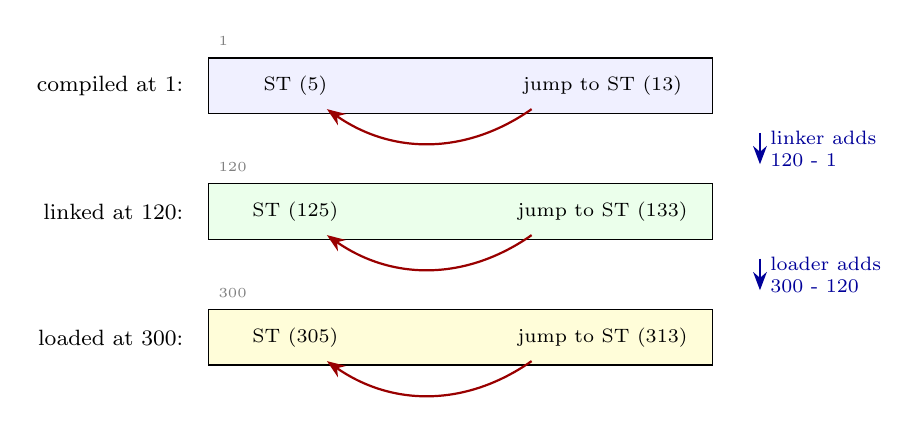
\begin{tikzpicture}[>=Stealth,font=\small,
 bar/.style={draw,minimum width=6.4cm,minimum height=0.7cm,fill=blue!6},
 lbl/.style={font=\footnotesize,anchor=east}]
\node[lbl] at (-0.2,1.6) {compiled at 1:};
\node[bar] (a) at (3.2,1.6) {};
\node[lbl] at (-0.2,0) {linked at 120:};
\node[bar,fill=green!8] (b) at (3.2,0) {};
\node[lbl] at (-0.2,-1.6) {loaded at 300:};
\node[bar,fill=yellow!15] (c) at (3.2,-1.6) {};
% positions within the bar: SUBR offsets 1..13 mapped to x
\foreach \y/\base in {1.6/1,0/120,-1.6/300} {
  \node[font=\tiny,gray,anchor=south west] at (0.0,\y+0.38) {\base};
}
\node[font=\scriptsize] at (1.1,1.6) {ST (5)}; \node[font=\scriptsize] at (5.0,1.6) {jump to ST (13)};
\node[font=\scriptsize] at (1.1,0) {ST (125)}; \node[font=\scriptsize] at (5.0,0) {jump to ST (133)};
\node[font=\scriptsize] at (1.1,-1.6) {ST (305)}; \node[font=\scriptsize] at (5.0,-1.6) {jump to ST (313)};
\draw[->,thick,red!60!black] (4.1,1.3) to[bend left=35] (1.5,1.3);
\draw[->,thick,red!60!black] (4.1,-0.3) to[bend left=35] (1.5,-0.3);
\draw[->,thick,red!60!black] (4.1,-1.9) to[bend left=35] (1.5,-1.9);
\draw[->,thick,blue!60!black] (7.0,1.0) -- node[right,font=\scriptsize,align=left]{linker adds\\120 - 1} (7.0,0.6);
\draw[->,thick,blue!60!black] (7.0,-0.6) -- node[right,font=\scriptsize,align=left]{loader adds\\300 - 120} (7.0,-1.0);
\end{tikzpicture}
\end{document}
